

%\documentclass[pra,twocolumn,epsfig,rotate,superscriptaddress,showpacs]{revtex4}


% \mathcal{u}se only LaTeX2e, calling the article.cls class and 12-point type.

\documentclass[prl,onecolumn]{revtex4-1}
\usepackage{graphicx}
\usepackage{epsfig}
\usepackage{epsf}
\usepackage{amssymb}
\usepackage{amsmath}
\usepackage{amsthm}
\usepackage{multirow}
\usepackage{hyperref}

\usepackage[framed,numbered]{matlab-prettifier}
\let\ph\snippetPlaceholder
\lstset
{
  style = Matlab-editor,
  escapechar      = ",
}

\renewcommand{\familydefault}{\sfdefault}  %% arial font
% \usepackage{times} %% times new roman font

\newcommand{\bra}[1]{\langle #1|}
\newcommand{\ket}[1]{|#1\rangle}

\newcommand{\be}{\begin{equation}}
\newcommand{\ee}{\end{equation}}
\newcommand{\bea}{\begin{eqnarray}}
\newcommand{\eea}{\end{eqnarray}}
\newcommand{\Fig}[1]{Fig.\,\ref{#1}}
\newcommand{\Eq}[1]{Eq.\,(\ref{#1})}
\newcommand{\la}{\langle}
\newcommand{\ra}{\rangle}
\newcommand{\nl}{\nonumber \\}
%\usepackage[usenames]{color}
%\definecolor{Red}{rgb}{1,0,0}
%\definecolor{Blue}{rgb}{0,0,1}




\setlength{\parindent}{0pt} % no incident
%\renewcommand{\baselinestretch}{1.2} % space between two lines
\setlength{\parskip}{6\lineskip} % space between two paragraphs

%%%%%%%%%%%%%%%%% END OF PREAMBLE %%%%%%%%%%%%%%%%



\begin{document}

% Include your paper's title here
\title{Notes on the 12 qubit PPS}
\author{Dawei Lu}

\begin{abstract}
Notes about the problems in the 12 qubit PPS preparation, including Matlab codes and Experiments.
\end{abstract}
\today

\maketitle

\section{Dec 12, 2014}

Calculating the state to state GRAPE on Ordi2. In pulsefinder folder. paramsfile is 'twqubit\_subS2S.m', and the output file is 'twqubit\_7zto12z'.

The GRAPE is to evolve ZZZZZZZIIIII to ZZZZZZZZZZZZ. As the couplings between nearest-neighbored C and H are about 150Hz. I set the GRAPE 

\begin{lstlisting}
% Number of timesteps
params.plength = 400;

% Length of each time step
params.timestep = 10e-6;

params.subsystem{1} = [1 2 3 9 10 11];
params.subsystem{2} = [4 5 6 7 8 12];
params.subsys_weight = [6 6];

% Input and goal states for state to state
params.rhoin = mkstate('+1ZZZZZZZIIIII',1);
params.rhogoal = mkstate('+1ZZZZZZZZZZZZ',1);

% Allow Zfreedom or not
params.Zfreedomflag = 1;
\end{lstlisting}

The fidelity keeps 0 all the time. Guess the reason is 'Zfreedom'. Set 'params.Zfreedomflag = 0;'. However, still 0.

Annie said maybe due to the length. Her SWAP gate requires 8ms, so I changed 'params.plength = 800;'. But for with or without Zfreedom, fidelity is still 0.

Check if some of my GRAPE settings are wrong. try to repeat Annie's SWAP gate calculation.

\begin{lstlisting}
% Number of timesteps
params.plength = 800;

% Length of each time step
params.timestep = 10e-6;

params.subsystem{1} = [1 2 3 9 10 11];
params.subsystem{2} = [4 5 6 7 8 12];
params.subsys_weight = [6 6];

% Input and goal states for state to state
params.rhoin = mkstate('+1IIIIIIIZIIII+1IIIIIIIIZIII+1IIIIIIIIIZII+1IIIIIIIIIIZI+1IIIIIIIIIIIZ',1);
params.rhogoal = mkstate('+1IIIIIIIZIIII+1IIIIIIIIZIII+1IIIIIIIIIZII+1IIIIIIIIIIZI+1IIIIIIZIIIIZ',1);

% Allow Zfreedom or not
params.Zfreedomflag = 0;
\end{lstlisting}

The outputfile is 'twqubit\_SWAPC7H5'. And the fidelity is already over 98\%.



%\begin{figure}[htb]
%\begin{center}
%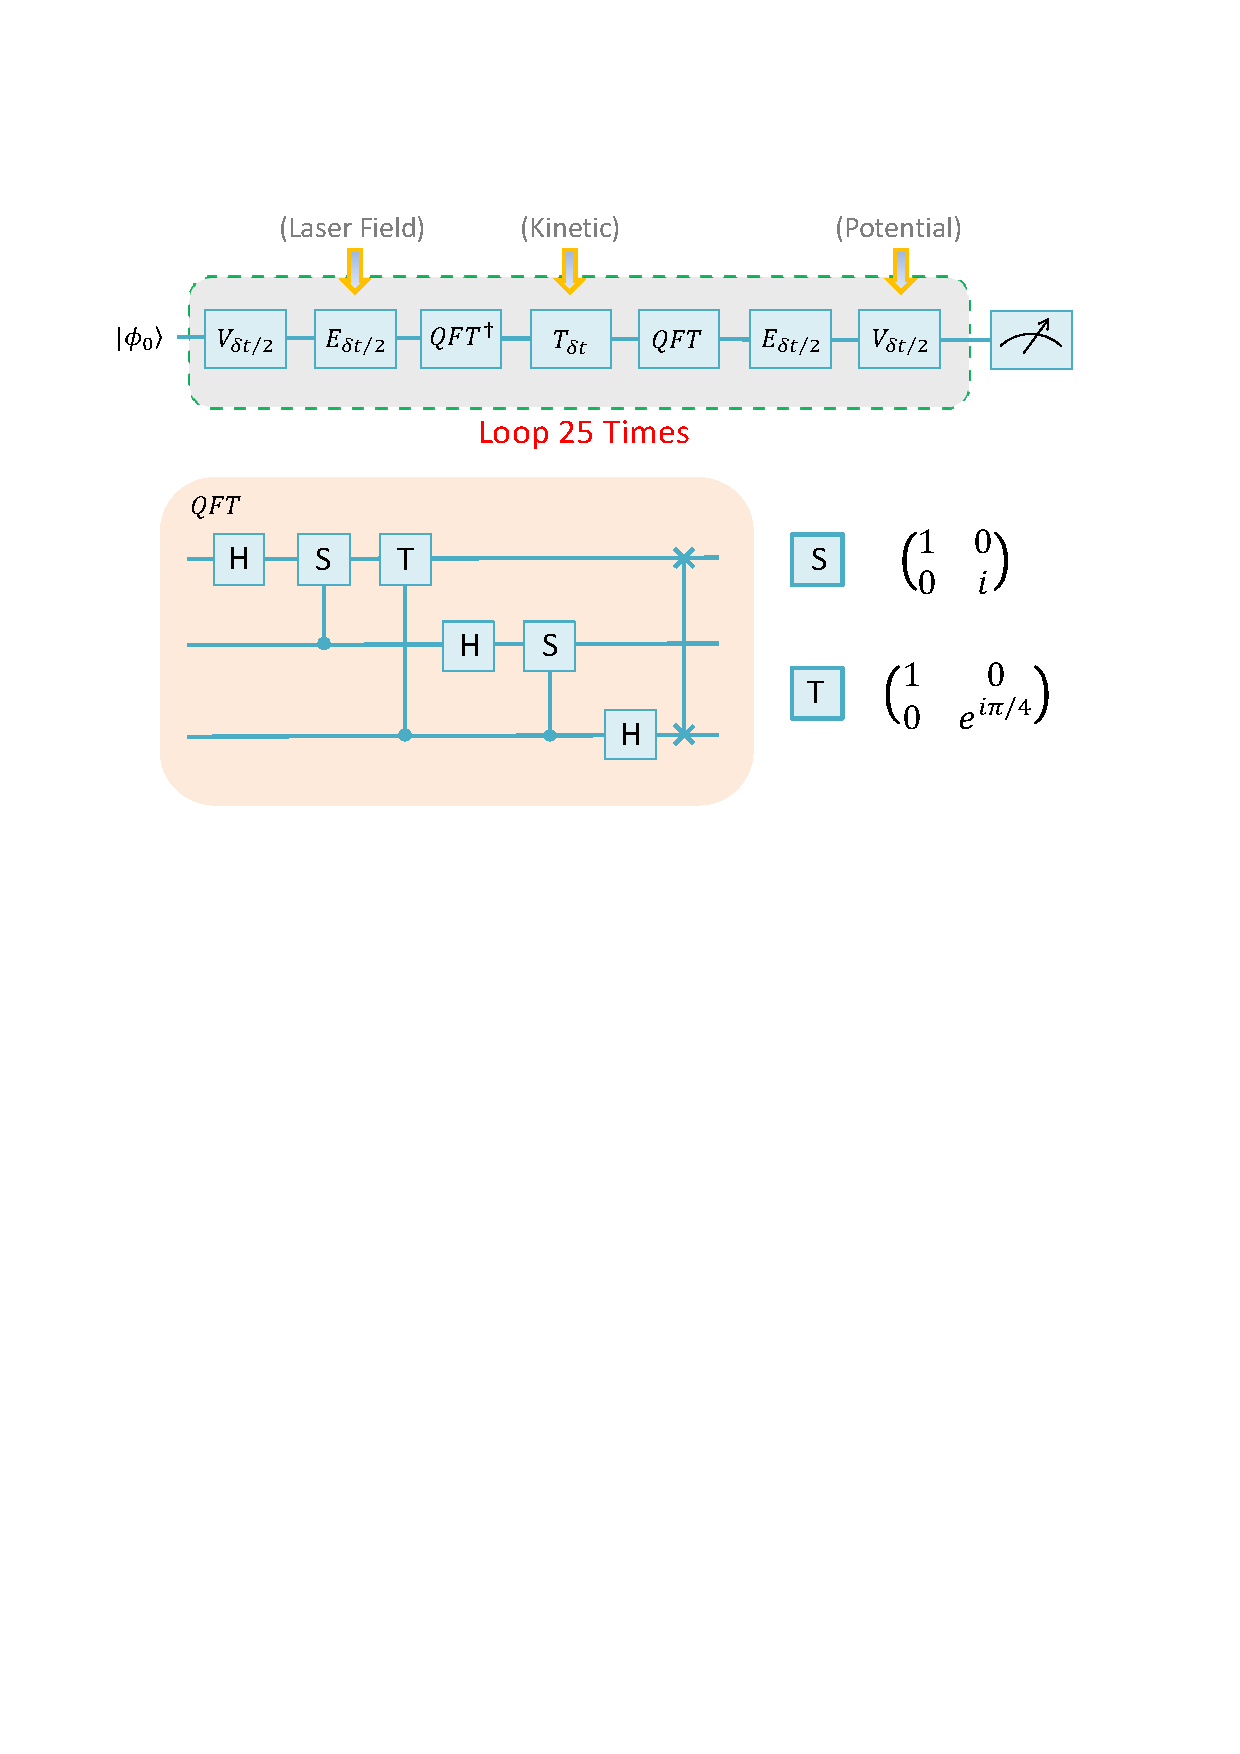
\includegraphics[width=\columnwidth]{circuit.pdf}
%\end{center}
%\setlength{\abovecaptionskip}{-0.35cm}
%\caption{\footnotesize{(color online). Circuit for twirling procedure based on the Clifford group $\mathcal{C}$. $\tilde{\mathcal{U}} = \Lambda \circ \mathcal{U}$ is the superoperator to describe the desired unitary $\mathcal{U}$ associated with some noise $\Lambda$. $M_\psi$ and $M_{\psi, \mathcal{C}_i, \mathcal{U}}$ are the original and modified measurement operators, respectively. In this protocol $\text{P}_1, \text{P}_2$ and $\text{P}_3$ are all Pauli operators and can be computed efficiently.}}\label{circuit}
%\end{figure}




\begin{thebibliography}{99}
%\bibitem{Moussa2012} O. Moussa, M. da Silva, C. Ryan, and R. Laflamme, Phys. Rev. Lett. \textbf{109}, 070504 (2012).

\end{thebibliography}


\end{document}
